\documentclass[handout,nooutcomes,noauthor]{ximera}

\graphicspath{  
{./}
{./whoAreYou/}
{./drawingWithTheTurtle/}
{./bisectionMethod/}
{./circles/}
{./anglesAndRightTriangles/}
{./lawOfSines/}
{./lawOfCosines/}
{./plotter/}
{./staircases/}
{./pitch/}
{./qualityControl/}
{./symmetry/}
{./nGonBlock/}
}


%% page layout
\usepackage[cm,headings]{fullpage}
\raggedright
\setlength\headheight{13.6pt}


%% fonts
\usepackage{euler}

\usepackage{FiraMono}
\renewcommand\familydefault{\ttdefault} 
\usepackage[defaultmathsizes]{mathastext}
\usepackage[htt]{hyphenat}

\usepackage[T1]{fontenc}
\usepackage[scaled=1]{FiraSans}

%\usepackage{wedn}
\usepackage{pbsi} %% Answer font


\usepackage{cancel} %% strike through in pitch/pitch.tex


%% \usepackage{ulem} %% 
%% \renewcommand{\ULthickness}{2pt}% changes underline thickness

\tikzset{>=stealth}

\usepackage{adjustbox}

\setcounter{titlenumber}{-1}

%% journal style
\makeatletter
\newcommand\journalstyle{%
  \def\activitystyle{activity-chapter}
  \def\maketitle{%
    \addtocounter{titlenumber}{1}%
                {\flushleft\small\sffamily\bfseries\@pretitle\par\vspace{-1.5em}}%
                {\flushleft\LARGE\sffamily\bfseries\thetitlenumber\hspace{1em}\@title \par }%
                {\vskip .6em\noindent\textit\theabstract\setcounter{question}{0}\setcounter{sectiontitlenumber}{0}}%
                    \par\vspace{2em}
                    \phantomsection\addcontentsline{toc}{section}{\thetitlenumber\hspace{1em}\textbf{\@title}}%
                     }}
\makeatother



%% thm like environments
\let\question\relax
\let\endquestion\relax

\newtheoremstyle{QuestionStyle}{\topsep}{\topsep}%%% space between body and thm
		{}                      %%% Thm body font
		{}                              %%% Indent amount (empty = no indent)
		{\bfseries}            %%% Thm head font
		{)}                              %%% Punctuation after thm head
		{ }                           %%% Space after thm head
		{\thmnumber{#2}\thmnote{ \bfseries(#3)}}%%% Thm head spec
\theoremstyle{QuestionStyle}
\newtheorem{question}{}



\let\freeResponse\relax
\let\endfreeResponse\relax

%% \newtheoremstyle{ResponseStyle}{\topsep}{\topsep}%%% space between body and thm
%% 		{\wedn\bfseries}                      %%% Thm body font
%% 		{}                              %%% Indent amount (empty = no indent)
%% 		{\wedn\bfseries}            %%% Thm head font
%% 		{}                              %%% Punctuation after thm head
%% 		{3ex}                           %%% Space after thm head
%% 		{\underline{\underline{\thmname{#1}}}}%%% Thm head spec
%% \theoremstyle{ResponseStyle}

\usepackage[tikz]{mdframed}
\mdfdefinestyle{ResponseStyle}{leftmargin=1cm,linecolor=black,roundcorner=5pt,
, font=\bsifamily,}%font=\wedn\bfseries\upshape,}


\ifhandout
\NewEnviron{freeResponse}{}
\else
%\newtheorem{freeResponse}{Response:}
\newenvironment{freeResponse}{\begin{mdframed}[style=ResponseStyle]}{\end{mdframed}}
\fi



%% attempting to automate outcomes.

%% \newwrite\outcomefile
%%   \immediate\openout\outcomefile=\jobname.oc
%% \renewcommand{\outcome}[1]{\edef\theoutcomes{\theoutcomes #1~}%
%% \immediate\write\outcomefile{\unexpanded{\outcome}{#1}}}

%% \newcommand{\outcomelist}{\begin{itemize}\theoutcomes\end{itemize}}

%% \NewEnviron{listOutcomes}{\small\sffamily
%% After answering the following questions, students should be able to:
%% \begin{itemize}
%% \BODY
%% \end{itemize}
%% }
\usepackage[tikz]{mdframed}
\mdfdefinestyle{OutcomeStyle}{leftmargin=2cm,rightmargin=2cm,linecolor=black,roundcorner=5pt,
, font=\small\sffamily,}%font=\wedn\bfseries\upshape,}
\newenvironment{listOutcomes}{\begin{mdframed}[style=OutcomeStyle]After answering the following questions, students should be able to:\begin{itemize}}{\end{itemize}\end{mdframed}}



%% my commands

\newcommand{\snap}{{\bfseries\itshape\textsf{Snap!}}}
\newcommand{\flavor}{\link[\snap]{https://snap.berkeley.edu/}}
\newcommand{\mooculus}{\textsf{\textbf{MOOC}\textnormal{\textsf{ULUS}}}}


\usepackage{tkz-euclide}
\tikzstyle geometryDiagrams=[rounded corners=.5pt,ultra thick,color=black]
\colorlet{penColor}{black} % Color of a curve in a plot



\ifhandout\newcommand{\mynewpage}{\newpage}\else\newcommand{\mynewpage}{}\fi

\title{Not so quick questions}


\author{Bart Snapp}

\begin{document}
\begin{abstract}
  Let's apply our knowledge.
\end{abstract}
\maketitle


\begin{listOutcomes}
\item 
\end{listOutcomes}


Imagine a house where the roof where two slopes meet. This will either
form a ``hip'' or a ``valley''.
\begin{center}
  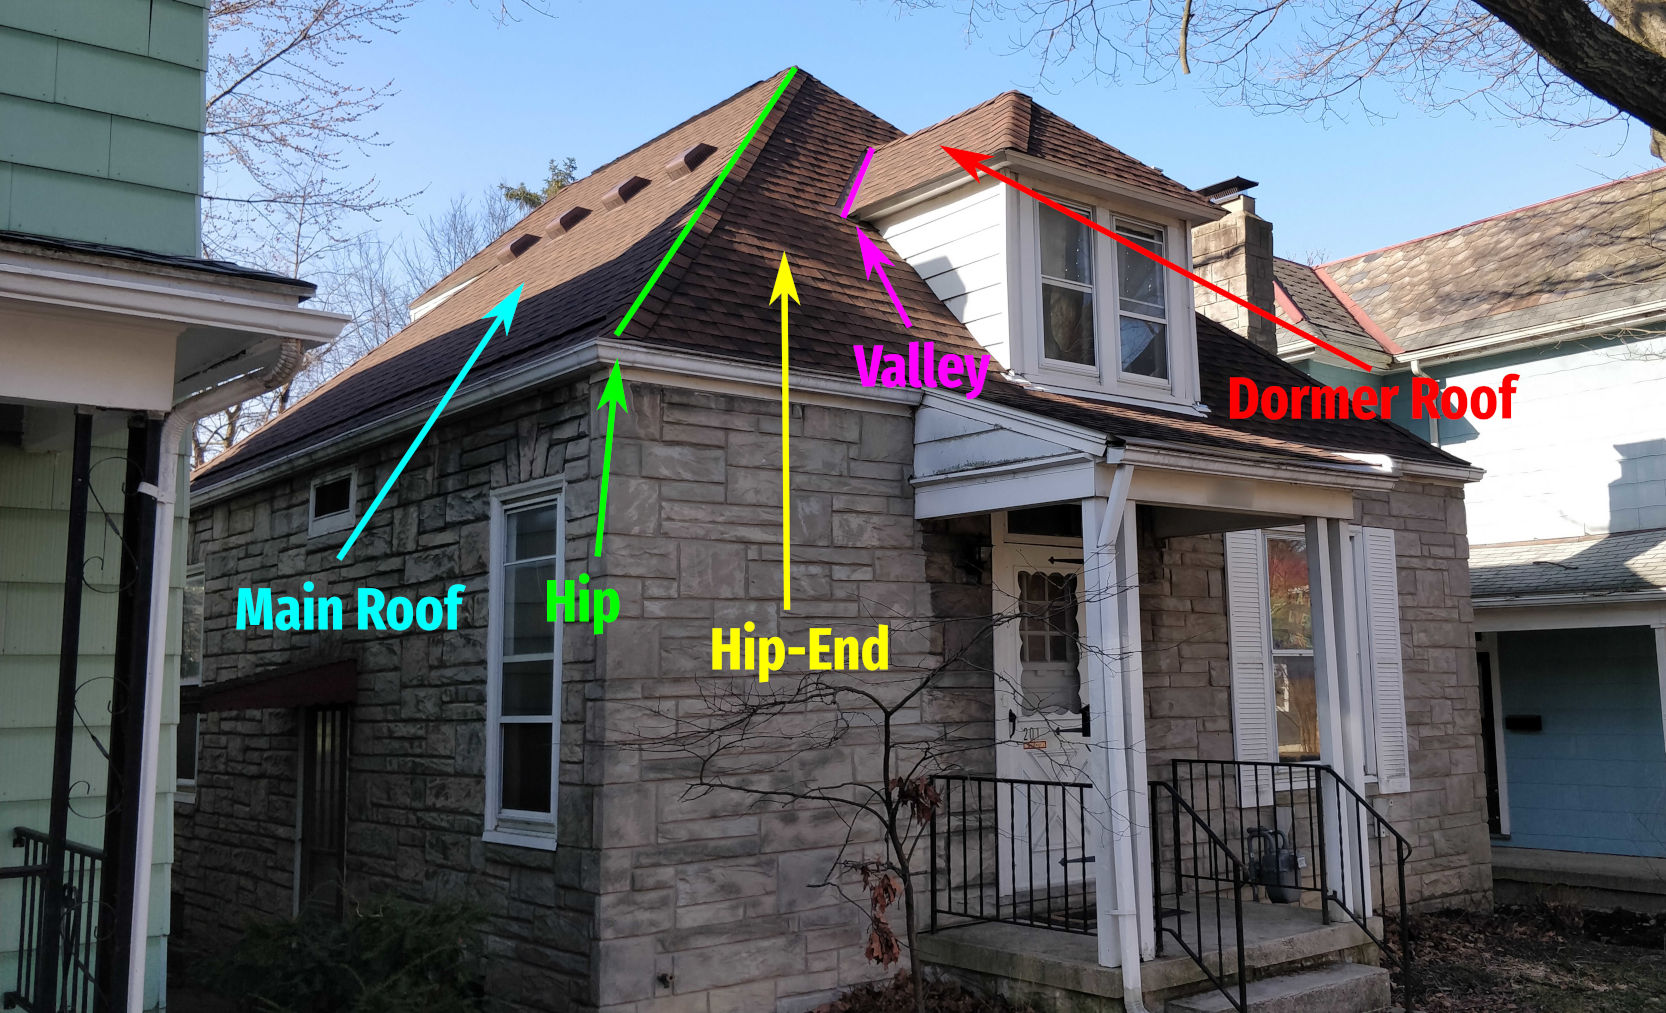
\includegraphics[width=.8\textwidth]{house.jpg}
\end{center}
We'd like to know the slope (or pitch) of the hip or valley. 
Let's use this:
\begin{quote}
  \textbf{Algorithm for computing the slope of a hip or valley:}

  Suppose the slopes are $\frac{s}{12}$ and $\frac{\l}{12}$ with
$s\le \l$.

\begin{enumerate}
\item Draw a point $O$ sitting at the intersection of a horizontal
  and vertical line.
\item Draw a vertical line segment $\bar{OS}$ where $S$ is directly
  above $O$ and $|OS| = s$.
  \item Starting from $S$, draw a line with the larger slope
    $\frac{\l}{12}$ and call the intersection of this line with the
    horizontal line point $X$.
  \item Starting at point $O$, extend the line segment $\bar{OS}$ by
    drawing downward $12$ units, and call the bottom of this segment
    $B$.
  \item The slope you seek is:
    \[
    \frac{|OS|}{|BX|}\qquad \text{with a pitch of} \qquad \frac{12\cdot |OS|}{|BX|}
    \]  
\end{enumerate}
        \begin{center}
        \begin{tikzpicture}[geometryDiagrams,scale=.2]
          %% \filldraw[black] (1in,1in) circle (2pt) ;
          %% \filldraw[black] (0in,0in) circle (2pt) ;
          %% \filldraw[black] (0in,1in) circle (2pt) ;
          %% \draw[<->,dashed] (1.5in,-.5in) -- (-.5in,1.5in);

          \tkzDefPoint(0,0){O}
          \tkzDefPoint(-13,0){I}
          \tkzDefPoint(1,0){nI}
          \tkzDefPoint(0,7){II}
          \tkzDefPoint(0,-13){nII}
          
          \tkzDefPoint(0,6){S}
          \tkzDefPoint(-9,0){X}
          \tkzDefPoint(-12,-2){BS}
          \tkzDefPoint(0,-12){B}

          \tkzDrawPoint[](O)
          \tkzDrawPoint[](S)
          \tkzDrawPoint[](X)
          \tkzDrawPoint[](B)
          \tkzDrawLine[ultra thin](II,nII)
          \tkzDrawLine[ultra thin](I,nI)
          \tkzDrawLine(S,BS)
          \tkzDrawSegment(O,B)
          \tkzDrawSegment[ultra thick](B,X)
          \tkzDrawSegment(O,S)

          \tkzLabelPoint(O){$O$}
          \tkzLabelPoint[](S){$S$}
          \tkzLabelPoint[above left](X){$X$}
          \tkzLabelPoint(B){$B$}

          \draw[decoration={brace,raise=.2cm,mirror},decorate,thin] (S)--(X);
          
          \node[anchor=south east] at (-5,4) {slope of $\frac{\l}{12}$};
        \end{tikzpicture}
      \end{center}
\end{quote}


\mynewpage

%% IDENTIFY OBIVIOUSLY CORRECT AND INCORRECT ANSWERS
%% AGAIN WITH THE AREA/VOL
%% solve a complex diagram
%% Give several quick questions and ask how they were supposed to figure them out.


%https://www2.strongtie.com/webapps/SlopeSkew/?source=app

%% EASY COMBINED PITCH
%% HARDER COMBINED PITCH
%% computer combined pitch
%% QUIZ: COULD IT JUST BE IS THIS A VALLEY OR A RIDGE?


\begin{question}
  Let's see if we can USE the algorithm above.
  \begin{enumerate}
  \item Someone used this drawing to compute the slope of a hip.
    \begin{center}
        \begin{tikzpicture}[geometryDiagrams,scale=.2]
          %% \filldraw[black] (1in,1in) circle (2pt) ;
          %% \filldraw[black] (0in,0in) circle (2pt) ;
          %% \filldraw[black] (0in,1in) circle (2pt) ;
          %% \draw[<->,dashed] (1.5in,-.5in) -- (-.5in,1.5in);

          \tkzDefPoint(0,0){O}
          \tkzDefPoint(-13,0){I}
          \tkzDefPoint(1,0){nI}
          \tkzDefPoint(0,7){II}
          \tkzDefPoint(0,-13){nII}
          
          \tkzDefPoint(0,6){S}
          \tkzDefPoint(-9,0){X}
          \tkzDefPoint(-12,-2){BS}
          \tkzDefPoint(0,-12){B}

          \tkzDrawPoint[](O)
          \tkzDrawPoint[](S)
          \tkzDrawPoint[](X)
          \tkzDrawPoint[](B)
          \tkzDrawLine[ultra thin](II,nII)
          \tkzDrawLine[ultra thin](I,nI)
          \tkzDrawLine(S,BS)
          \tkzDrawSegment(O,B)
          \tkzDrawSegment[ultra thick](B,X)
          \tkzDrawSegment(O,S)


          \draw[decoration={brace,raise=.2cm,mirror},decorate,thin] (O)--(S);
          \node[anchor=west] at (1.5,3) {$6$};


          \draw[decoration={brace,raise=.2cm,mirror},decorate,thin] (B)--(O);
          \node[anchor=west] at (1.5,-6) {$12$};

          \draw[decoration={brace,raise=.2cm,mirror},decorate,thin] (S)--(X);
          \node[anchor=south east] at (-5,4) {slope of $\frac{8}{12}$};

          \draw[decoration={brace,raise=.2cm,mirror},decorate,thin] (X)--(B);
          \node[anchor=north east] at (-5,-6.5) {$15$};
        \end{tikzpicture}
    \end{center}
    Find the slopes of the main-roof, the hip-end, and the hip. Show
    all work and explain your reasoning.
  \item Suppose you have a main-roof with a slope of $\frac{4}{12}$
    and a hip-end with a slope of $\frac{7}{12}$. \textbf{Find the
      slope of the hip.}  Show all work and explain your reasoning and
    check your work with an online calculator.
  \end{enumerate}
\end{question}




\mynewpage


\begin{question}
  Now make them explain it.
\end{question}

\mynewpage


\begin{question}
  FINALLY -- compute two SA

  1) Pyramid los

  2) roof with hips etc
\end{question}


\end{document}
